\documentclass[a4paper,11pt,notitlepage]{article}

\usepackage{amsfonts}
\usepackage{amsmath}
\usepackage{amsthm}
\usepackage{amssymb}
\usepackage{graphicx}
\usepackage{rotating}

\usepackage{fontspec}
\defaultfontfeatures{Mapping=tex-text}
\setmainfont{Times New Roman}

\usepackage{fullpage}

\usepackage[american]{babel}
\usepackage{csquotes}
\usepackage[style=apa,natbib=true,backend=biber]{biblatex}
\DeclareLanguageMapping{american}{american-apa}
\addbibresource{Polarization.bib}

\usepackage[colorlinks,allcolors=blue]{hyperref}
\hypersetup{%
    pdftitle={Is Technology Polarizing the Australian Work Force?},%
    pdfauthor={Alex Cooper},%
    pdfsubject={An analysis of one determinant of inequality in Australia.},%
    pdfkeywords={labor, polarization, routinization, SBTC, inequality},%
}
\ExecuteBibliographyOptions{doi=false}
\newbibmacro{string+doi}[1]{%
  \iffieldundef{doi}{#1}{\href{http://dx.doi.org/\thefield{doi}}{#1}}}
\DeclareFieldFormat{title}{\usebibmacro{string+doi}{\mkbibemph{#1}}}
\DeclareFieldFormat[article]{title}{\usebibmacro{string+doi}{\mkbibquote{#1}}}
\renewcommand{\bibfont}{\normalfont\small}

\usepackage[font=small,format=plain,labelfont=bf,up,textfont=it,up]{caption}

\renewcommand{\H}{\mathcal{H}}
\renewcommand{\L}{\mathcal{L}}

\title{Is Technology Polarizing the Australian Work Force?}
\author{Alex Cooper \\
        Honors Candidate \\
        Macquarie University}
\date{August, 2013}

\begin{document}

\vspace{6cm}

\maketitle

\vspace{3cm}

\begin{abstract}Could technology be responsible for part of the rise of income inequality over the past 30 years?
This research is motivated by the fact that, while technology can make workers more productive, it also has the capacity to put others out of work entirely. We proceed in two parts. First, we consider the standard model of skill-biased technical change, and show that it explains some, but not all, of the trends observed in the data. We then take an alternative approach by considering the task content of occupations, an approach that has been used with success in foreign labor markets. We perform a simple, preliminary test of the relationship between technology investment and polarization, and find a negative relationship between the wage share of middle-skilled workers, and investment in electronic and electrical capital goods.
\end{abstract}

\clearpage

\section{Motivation}
The income distribution for Australian workers has widened over the past 30 years. Although there are many possible developments that explain this trend, we focus on just one: the rapid rise of technology in the work force. We first consider the standard model of skill-biased technical change, and show that it explains some, but not all, of the trends observed in the data. We then consider an alternative approach, following \citet{Levy2003}, which has been used with success in foreign labor markets, and perform a simple preliminary test of the relationship between investment and polarization.

The second half of the 20th century has witnessed tremendous change for Australian workers. Since 1973, average real per capita incomes have approximately doubled \citep{NA20124}, and the number of jobs has increased by over three million \citep{LFSApr2013}. During the same period, top percentile wage growth has far outstripped that of lower-wage earners \citep{Atkinson1997,Borland1999}. And although income inequality in Australia fell somewhat between the 1950's and 1970's, it has since risen consistently for the last 30 years \citep{Leigh2005,Gaston2009}.

There is a large literature studying the rise of wage inequality in Australia. Empirical studies have confirmed that both individual-level and household-level inequality have been rising since the 1980s \citep{Borland1999,Leigh2005,Gaston2009}. A number of studies exist on the task content of Australian jobs \citep{Esposto2012a}, and the change over time of the skill intensity of various professions \citep{Esposto2012, Esposto2012a}. Although ICT use and globalization have been found to Granger (non-)cause rising inequality \citep{Gaston2009}, no studies have tested whether workers' skill allocation is the channel through which this change has occurred.

Although mechanical computers and computation aids (the abacus, for instance), have been available for centuries, it was only in the post-war era, with the arrival of electronic computation, that the price of computation began to fall dramatically. \citet{Nordhaus2007} estimates that, between 1946 and 2006, the cost per computation decreased by a factor of {\em seven trillion,} and over the same period, the cost of data storage fell at a comparable rate. The falling cost of computation opened up new avenues for research in information technology, so that even as computation became cheaper, new and improved algorithms were developed which made more efficient use of, and found novel uses for, computing power. And as computers have become cheaper and more useful, firms have made greater use of them. Between 1981 and 2012, Australian firms' real annual investment in computers has grown from \$26M to \$14B.\footnote{ABS National Accounts, cat. no. 5204.0. 2012 dollars.}

\section{Skill-biased technical change}

A leading explanation for this divergence of incomes is that skilled work and new technologies are complements in production, or factor augmenting. This idea, developed by \citet{Tinbergen1974}, \citet{Katz1992} and others, suggests that new workplace technologies disproportionately complement highly-skilled technical and managerial jobs, relative to low-skilled manual and service jobs. Under this explanation, the premium paid to high-skilled labor increases for two reasons: first, since high-skilled workers become relatively more productive, wages to high-skilled occupations are higher at the margin. There is also evidence that, in the United States at least, an increase in the demand for skilled labor, relative to its supply, has resulted in higher wages for skilled occupations. In the jargon, such technologies are said to exhibit \emph{skill bias} \citep{Autor2006}.

We will take as a point of departure the standard model for analyzing skill-based technical change (SBTC). This model, dubbed the `canonical' model by \citet{Acemoglu2011} and which has sparked a voluminous literature, has enjoyed considerable empirical success explaining rising wages for high-skill managerial and professional jobs in the United States and Europe \citep{Katz1992}. Since the canonical model includes \emph{factor-augmenting} capital, it predicts a uniform skill upgrading of the work force at all education levels \citep{Levy2003}. Skill upgrading has been confirmed by a number of authors, both in Australia \citep{Esposto2012, Wooden2000, Cully1999} and overseas \citep{Autor2008}. 

Consider a competitive economy with two different, imperfectly substitutable types of labor: high-skilled and low-skilled.\footnote{This section follows the notation employed by \citet{Acemoglu2011}.} Workers are heterogeneous, with different levels of efficiency within each skill group. Let the total supply of high-skilled labor be $H$, and the total supply of low-skilled labor be $L$, and both types are paid the same wage, respectively $w_h$ and $w_\ell$. Production in this economy is governed by a CES aggregate production function, with elasticity of substitution $\sigma$, where $\sigma>1$:
\begin{equation}  \label{eq:prod}
Y = \left[
  \left(A_LL \right)^\frac{\sigma-1}{\sigma}
  +
  \left(A_HH \right)^\frac{\sigma-1}{\sigma}
  \right]^\frac{1}{\sigma-1}.
\end{equation}

For our purposes, we are interested in two claims about relative wages made by this model: first, that technological change or a generalized shift from low-skilled to high-skilled work should never cause low-skilled wages to decrease, and second, that technological change should result in a monotonic increase in wage across the skill spectrum. To see this, we will first derive the expressions for the equilibrium wage for each type of labor. Since the economy is competitive, unique equilibrium wages for both both high- and low-skilled workers are given by their respective marginal products. Wages can therefore be found by differentiating \eqref{eq:prod} with respect to labor supply:
\begin{align}
w_h &= \frac{\partial Y}{\partial H} 
     = A_H^\frac{\sigma-1}{\sigma}\left(
              A_L^{\frac{\sigma-1}{\sigma}} (H/L)^{-\frac{\sigma-1}{\sigma}} + A_H^{\frac{\sigma-1}{\sigma}}
        \right)^{\frac{1}{\sigma - 1}} \label{eq:wh} \\
w_l &= \frac{\partial Y}{\partial H} 
     = A_L^\frac{\sigma-1}{\sigma}\left(
              A_L^{\frac{\sigma-1}{\sigma}} + A_H^{\frac{\sigma-1}{\sigma}}(H/L)^{\frac{\sigma-1}{\sigma}}
        \right)^{\frac{1}{\sigma - 1}} \label{eq:wl}
\end{align}
The first claim follows from differentiating these wage equations. First, notice in \eqref{eq:wl} that $\partial w_L/\partial A_H \geq 0$. This means that, in this model, an increase in technology for high-skilled workers does not reduce the wage for low-skilled workers. Technological progress should in fact result in positive wage improvements for both high- and low-skilled workers. 

Next, notice that $\partial w_l/\partial(H/L)>0$. An increase in the relative supply of high-skilled workers, $H/L$, should therefore not decrease the wage of low-skilled workers. Rather, as high-skilled work becomes more productive and the ratio of skilled to unskilled workers increases, the demand for low-skilled work simultaneously increases. 

Second, consider the ratio between high- and low-skilled labor, $\omega=w_h/w_l$ (for convenience, we will consider the log ratio.) It is straightforward to show that this ratio depends on the state of technology and labor inputs:
\begin{equation}\label{eq:omega}
\log \omega = \frac{\sigma-1}{\sigma}\log\left(\frac{A_H}{A_L}\right) - \frac{1}{\sigma}\log\left(\frac{H}{L}\right).
\end{equation}
This equation illustrates the two countervailing forces of Tinbergen's (1974) `race' for education that govern the magnitude of the skill premium. Holding the labor supply ratio constant, and recalling our assumption that $\sigma >1$, an increase in skill-biased technology $A_H/A_L$ results in a larger $\log\omega$. On the other hand, holding technology constant, an increase in the proportion of workers providing high-skilled labor should decrease the log skill premium.\footnote{Formally, $\partial \log\omega / \partial(A_H/A_L) > 0$, and 
$\partial \log\omega / \partial(H/L) < 0$.} In this model, a rising skill premium occurs when the first term of \eqref{eq:omega}  dominates the second.

To review, the SBTC model claims that unless there is technical regress, wages for all skill types will always increase, and never decrease (wages should follow a monotonic path.) Second, in the presence of an increasing proportion of workers conducting skilled work, the model is consistent with either a rising or a falling log skill premium.

\subsection{Data}

To bring the SBTC model to the data, we employ the Survey of Income and Housing, a hierarchical clustered household survey conducted by the ABS every 2-3 years since 1995, and also for the fiscal years 1985-6 and 1981-2. The survey provides detailed  information about respondents' labor and non-labor income sources, as well as data on age, educational attainment, hours worked and industry and occupation. For the surveys conducted between 2000 and 2010, as well as the 1981-2 survey, the data include detailed occupational data, which will become important later. The other surveys include occupation only at the one-digit level. We obtain survey micro-data as confidentialized unit record files (CURFs).

To facilitate inter-temporal comparisons, we must eliminate effects which arise as a result of mechanical, demographic shifts. Between 1982 and 2010, the number of women in the work force has increased dramatically, and the same period has seen an evolution of the educational and age composition of the work force, and the rate of casual and part-time employment has increased. Following \citet{Acemoglu2011}, we therefore include only full-time workers for whom labor forms the primary source of income. We further composition-adjust each survey to match 2010 demographics by linearly scaling the survey selection weights for each age group/sex/educational group cell. All computations in this study treat these adjusted weights as inverse selection probabilities.

\begin{figure}
  \centering
  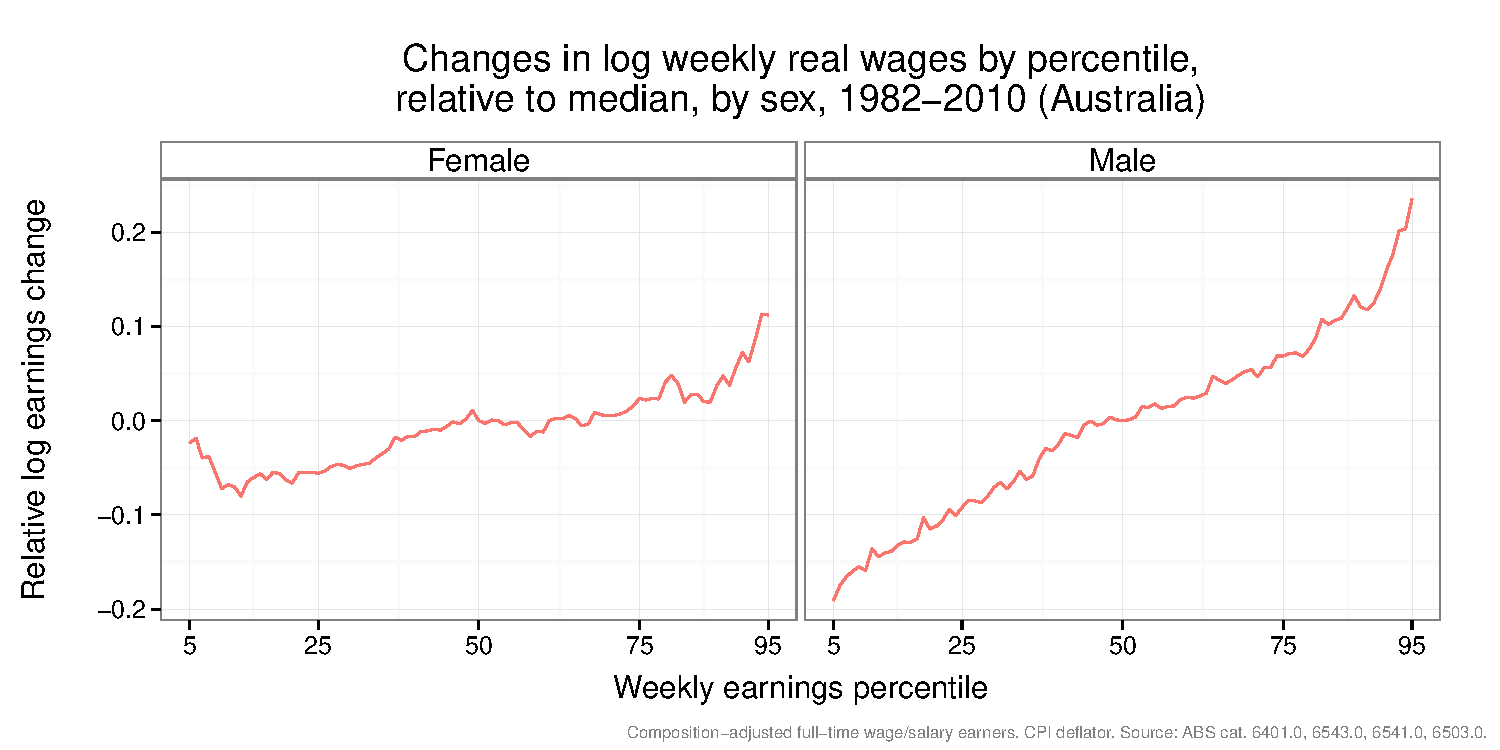
\includegraphics[width=\textwidth]{../figure/quantile_mf.pdf}
  \caption{Change in weekly wage by percentile, 1981-2010, Males and Females. Full-time workers whose main sources of income are wages and salaries are shown. Notice that real wage growth has been non-monotone for males in lower percentiles. Source: Survey of Income and Housing.}
  \label{fig:banana}
\end{figure}

\subsection{Does SBTC fit the Australian data?}

If SBTC explained the widening of the income distribution, we would expect to observe the premium accruing to `skilled' labor increasing with time. Figure~\ref{fig:banana} shows the composition-adjusted changes in log real wage by percentile, for males and females, between 1981-82 and 2009-10. If the 1981-82 income percentile can be considered a proxy for skill, then it is apparent that, over this period, wages more grew for high-skill individuals much faster than for low-skill individuals. It would therefore be expected that the premium accruing to higher educational attainment would show a similar trend.

In the United States, at least, the wage premium earned by tertiary-educated labor fell in the 1970s, but has risen each decade since then \citep{Acemoglu2011}. \citet{Katz1992} employs a similar empirical model which explains the rise of the skill premium in the United States in the post-war era. In Australia, however, a corresponding growth in the premium for tertiary qualifications has not been observed. Table~\ref{tbl:wagepremium} shows the log skill premium for Australia and the United States between 1982 and 2008. Rather than any fundamental differences in the nature of the demand for skills, \citet{Coelli2009} attributes this difference in Australian workers to differences in the nature of Australian educational qualifications. In Australia, University degrees are available to a wider range of candidates and for a wider range of disciplines than those who would traditionally have undertaken university studies in the United States. As a result, tertiary educational attainment may be a poor proxy for `skilled' work in Australia.
\begin{table}
  \centering
  \begin{tabular}{lcc}
  \hline
           & \multicolumn{2}{c}{\bf Log Skill Premium} \\
\hline
{\bf Year} &	{\bf United States} & {\bf Australia} \\
{\bf 1982} &	0.42 &	0.42 \\
{\bf 1995} &	0.59 &	0.36 \\
{\bf 2003} &	0.64 &	0.37 \\
{\bf 2008} &	0.68 &	0.34 \\ \hline
\end{tabular}
  \caption{University/non-university log wage premium, Australia and the United States. The figures show the difference between the mean log weekly income for workers who have attained a bachelor degree or higher, and the mean weekly income of other workers. Only full-time workers whose main sources of income are wages and salaries are included, and survey data have been composition adjusted for sex, age group, (and for the United States, race). Source: for Australia, ABS Survey of Income and Housing, and for the United States, \citet{Acemoglu2011}.}
  \label{tbl:wagepremium}
\end{table}

The SBTC model also claims that, even if technology exhibits skill bias, wages for all skill groups should increase monotonically. Figure~\ref{fig:changetime} plots the cumulative change over time for three wage percentiles, the 5th, 95th, and the median. Over the period 1981-82 to 2009-10, although wages at the top percentiles increased steadily, the same is not true for the lower percentiles. Indeed, for all of the 1990s and much of the 2000s, cumulative real income growth from 1981-82 was negative for many workers.
\begin{figure}
  \centering
  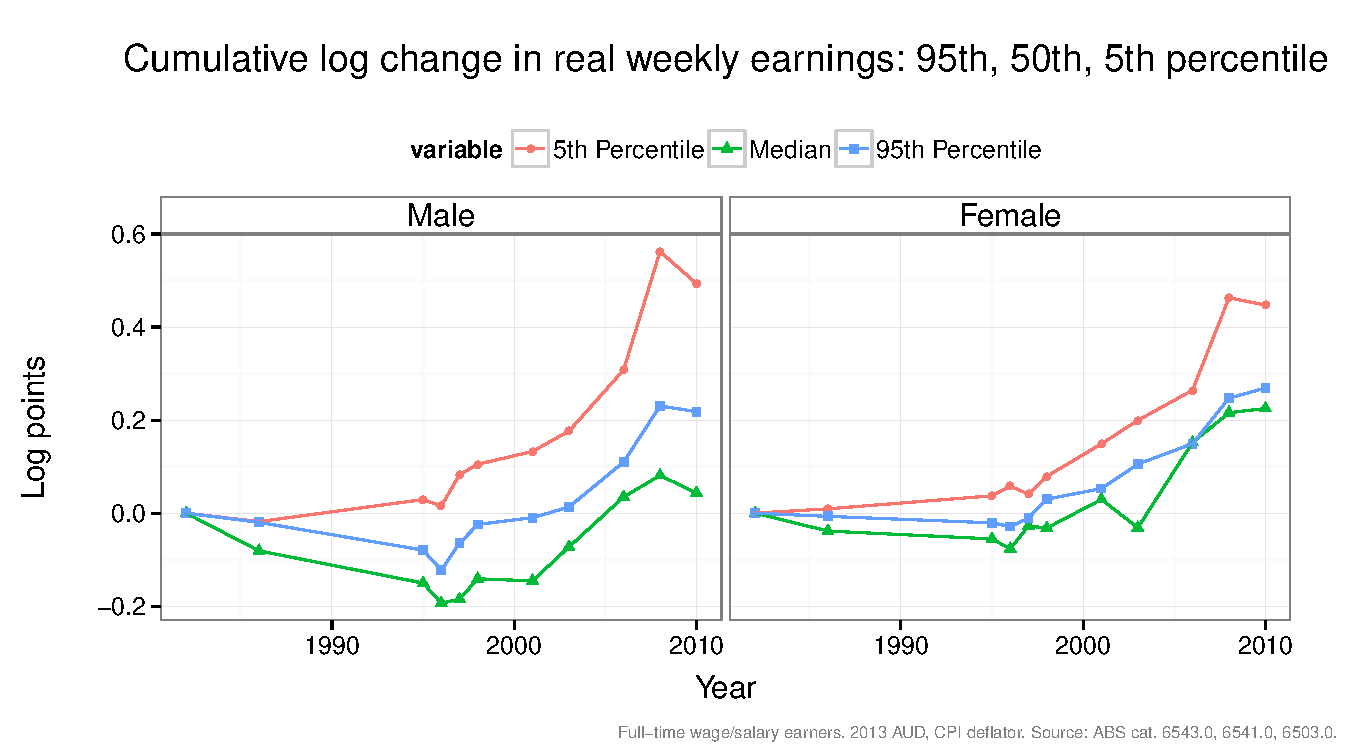
\includegraphics[width=\textwidth]{../figure/wage_change_time.pdf}
  \caption{Cumulative log change in real weekly earnings, 5th, 50th and 95th percentiles, 1982-2010. Full-time workers whose main sources of income are wages and salaries are shown. Notice that real wage growth has been non-monotone for males in lower percentiles. Source: Survey of Income and Housing.}
  \label{fig:changetime}
\end{figure}

That the income distribution is widening, but the skill premium is {\em not} driving the change, suggests one of at least two interpretations. We have already discussed the fact that educational attainment may be a poor indicator of skill for the Australian labor market. A second, more nuanced explanation was given by \citet{Levy2003}. Technological change may not be complementary to all types of labor; it may replace many types of labor entirely.

\section{An alternate approach: `jobs' and `tasks'}

% flabby
Since the late 1990s, both in Europe and the United States, the data show a marked polarization in the work force \citep{Goos2007, Autor2006}. This polarization has simultaneously manifested in \emph{wages} and in \emph{jobs}: both wage growth and growth in the level of employment are concentrated in high-skill jobs, and to a lesser extent, the bottom end of the skill spectrum. Middle-skill jobs have stagnated since the 1990s, both in terms of remuneration and level. The recent rise of ICT investment by firms has been attributed for this trend, both because many middle-skilled jobs can be substituted by computer capital, and because communications technologies enable firms to out source non-customer-facing roles to remote locations in order to take advantage of cheaper labor.

Computers, despite their sophistication, are only capable of performing a very limited set of simple, routine tasks. They excel at processes which require calculation and simple symbolic manipulation, and are not prone to the same types of errors as human workers. It is this fact which has led to their widespread adoption in automated tellers and a wide range of electronic service delivery which were formerly the domain of human personnel. Yet, any task that requires abstract thought or physical coordination, however elementary it may appear to a human worker, is not yet possible with a machine. Under this definition, many occupations which we might colloquially consider `routine'---such as stacking shelves or driving a taxi---require a degree of perception and motor control out of reach for a computer, and for our purposes are `non-routine.' In these areas, for the moment at least, human workers enjoy a competitive advantage, and technology is not yet a substitute \citep{Levy2003}.

Thus computing capital is a complement to some kinds of task-performing labor, and a substitute for others. As \citet{Levy2003} show, in the United States between 1960 and 1998, computerization led to a substitution in the observed levels of employment, away from routine tasks and toward cognitive tasks. Non-routine tasks, on the other hand, may improve, rather than replace, the efficiency of human workers. Indeed, as \citet{Borland2004} found by studying the computer knowledge of a cross-section of Australian workers surveyed in 1992, computer knowledge accrues a skill premium of around 10\%. Likewise, \citet{Goos2007} show a similar trend in the United Kingdom: between 1975 and 2003, they find an increase in the number of ``lovely'' (high-skill, high-wage) jobs and ``lousy'' (low-wage, low-skill) jobs, but a relative decrease in the number of ``middling'' jobs. In a subsequent paper, a similar pattern was found for most of Continental Europe \citep{Goos2009}.

The task approach departs from the standard neoclassical production function, which views aggregate economic output as a simple function of inputs such as capital and labor, but does not consider the specifics of the processes which produced that output \citep{Acemoglu2011}. Although the canonical approach has been very successful in explaining aggregate output levels, it is not sensitive to qualitative changes in the nature of production such as changes in the technology which produce output. 

\subsection{A simple test of the task approach}

To test this pattern for Australian data, we can augment \eqref{eq:prod} by introducing a third type of labor, $M$, to represent work which requires mid-level skill and low levels of physical activity, representing `routine' or `middling' work. We also introduce computer capital, $C$, as a substitute in production for medium-skilled labor, and a complement in production for high-skilled workers:
\begin{equation}  \label{eq:prod2}
Y = \left[
  \left(A_LL \right)^\frac{\sigma-1}{\sigma}
  +
  \left(A_MM + C\right)^\frac{\sigma-1}{\sigma}
  +
  \left((A_HH)^\mu + C^\mu\right)^\frac{\sigma-1}{\mu\sigma}
  \right]^\frac{1}{\sigma-1}.
\end{equation}
\citet{Michaels2010} use a formulation similar to \eqref{eq:prod2} to show that, if ICT investment $C$ increases exogenously, the wage share for high-skill workers should increase, but decrease for low-skill workers. Likewise, the wage premium for high-skilled workers should rise with increasing ICT investment, and fall for medium-skilled workers.\footnote{Following \citet{Michaels2010}, we focus on the wage {\em share}, and not the absolute wage. Although wages for high-skilled and low-skilled workers should increase with increased investment, the comparative static predictions for medium-skilled workers are indeterminate. Michaels et al. prove that the comparative static predictions for the wage share, however, are unambiguous.} To test these predictions, \citet{Michaels2010} specify a simple translog flexible functional form to test the impact of ICT investment on the wage share for type of labor $S\in\{H,M,L\}$, estimated for broad industry groups across eleven countries, using educational attainment as a proxy for skill. The authors find support for the claim that ICT investment is associated with a decrease in the demand for middle-skilled labor. 

Adapting their specification for Australia gives the empirical model shown below. In this model, $SHARE^S$, computed as ${\sum_k W^S_k/\sum_{s,j}W^s_j}$ is the wage bill share for the labor category $S$, $C$ is ICT capital, $K$ is non-ICT capital, and $Q_i$ is value added by industry $i$. 
\begin{equation} \label{eq:translog}
\Delta SHARE^S = \alpha_{CS}\log(C/Q)_{it} + \alpha_{KS}\log(K/Q)_{it} + \alpha_{QS}\log(Q)_{it}.
\end{equation}
As Michaels {\it et al.} point out, the polarization hypothesis is consistent with $\alpha_{MS}<0$ and $\alpha_{HS}>0$.

With the results from the previous section in mind, to adapt this specification for Australia requires an alternative yard-stick for `skill.' Following \citet{Levy2003}, we partition occupations according to the tasks they involve, according to the occupational classification coded in the SIH. For the purposes of this very simple and informal model, we divide occupations into three categories: `non-routine manual' (low-skilled), `routine' (middle-skilled), and `non-routine cognitive' (high-skilled.) Capital series were derived from national accounting data. Our data include two different measures of ICT capital: {\em software}, and {\em electrical and electronic equipment}. Software includes both commercial off-the-shelf packages, as well as custom-built line-of-business programs, whereas the second variable includes telecommunications equipment and other electronic machinery. To smooth out variation in the data, the  period 1996-2010 was divided into two seven-year periods.

\subsection{Results}

The results from estimating \eqref{eq:prod2}, given in Table~\ref{tbl:reg}, lend mixed support for the polarization hypothesis. While estimates for $\alpha_{MS}<0$ and $\alpha_{HS}>0$ have the expected sign, they are not significant when estimated with all the parameters specified in $\eqref{eq:translog}$. However, with just electrical and electronic equipment included in regression, $\alpha_{MS}<0$ is negative and significant at the 5\% level. Column (4) of Table~\ref{tbl:reg} suggests that, over a seven-year period, a 10\% increase in electrical and electronic equipment capital is associated with a decrease in the wage share of middle-skilled workers of around 0.2, whereas it is associated with a relative increase in the wage share of high-skill workers versus low-skilled workers.

The sign of coefficient estimates for the {\em software} variable are opposites in all estimates. This suggests that software capital may in fact be a complement to medium-skilled labor. Since {\em equipment} includes telecommunications infrastructure, one interpretation is that {\em outsourcing}, rather than a direct application of labor-saving capital, is responsible for the decline in middle-skill labor.

\begin{sidewaystable} \begin{center}
  \caption{Wage Share Change Estimation Results: 1996-2010} 
  \label{tbl:reg} 
\begin{tabular}{@{\extracolsep{5pt}}lcccccc} 
\\[-1.8ex]\hline 
\hline \\[-1.8ex] 
 & \multicolumn{6}{c}{\textit{Dependent variable:}} \\ 
\cline{2-7} 
\\[-1.8ex] & \multicolumn{2}{c}{$\Delta SHARE^H$} & \multicolumn{2}{c}{$\Delta SHARE^M$} & \multicolumn{2}{c}{$\Delta SHARE^L$} \\ 
\\[-1.8ex] & (1) & (2) & (3) & (4) & (5) & (6)\\ 
\hline \\[-1.8ex] 
 $\Delta$log {\em equipment} & 0.037 & 0.081 & $-$0.144 & $-$0.249$^{**}$ & 0.107 & 0.169$^{*}$ \\ 
  & (0.100) & (0.080) & (0.108) & (0.094) & (0.099) & (0.084) \\ 
  & & & & & & \\ 
 $\Delta$log {\em software} & $-$0.018 &  & 0.109$^{*}$ &  & $-$0.091$^{*}$ &  \\ 
  & (0.052) &  & (0.056) &  & (0.052) &  \\ 
  & & & & & & \\ 
 $\Delta$log {\em other capital} & 0.118 &  & $-$0.173 &  & 0.055 &  \\ 
  & (0.176) &  & (0.191) &  & (0.176) &  \\ 
  & & & & & & \\ 
 $\Delta$log {\em value added} & 0.113 & 0.071 & 0.035 & 0.030 & $-$0.148 & $-$0.102 \\ 
  & (0.163) & (0.127) & (0.176) & (0.149) & (0.163) & (0.133) \\ 
  & & & & & & \\ 
 Constant & 0.040 & 0.055 & $-$0.102 & $-$0.095 & 0.062 & 0.040 \\ 
  & (0.073) & (0.060) & (0.079) & (0.070) & (0.073) & (0.063) \\ 
  & & & & & & \\ 
\hline \\[-1.8ex] 
Observations & 30 & 30 & 30 & 30 & 30 & 30 \\ 
R$^{2}$ & 0.068 & 0.044 & 0.343 & 0.210 & 0.251 & 0.151 \\ 
Adjusted R$^{2}$ & $-$0.081 & $-$0.026 & 0.238 & 0.152 & 0.132 & 0.089 \\ 
Residual Std. Error & 0.101 (df = 25) & 0.098 (df = 27) & 0.109 (df = 25) & 0.115 (df = 27) & 0.101 (df = 25) & 0.103 (df = 27) \\ 
F Statistic & 0.455 (df = 4; 25) & 0.627 (df = 2; 27) & 3.268$^{**}$ (df = 4; 25) & 3.593$^{**}$ (df = 2; 27) & 2.100 (df = 4; 25) & 2.409 (df = 2; 27) \\ 
\hline 
\hline \\[-1.8ex] 
\textit{Note:}  & \multicolumn{6}{r}{$^{*}$p$<$0.1; $^{**}$p$<$0.05; $^{***}$p$<$0.01} \\ 
\normalsize 
\end{tabular} 
\end{center}
{\em Wage shares computed for full-time workers, whose primary sources of income are wages and salaries, estimated for 16 industry groups. `High skill' workers include professionals and managers, `middle skill' workers include sales persons, clerical workers and para-professionals, and `low skill' workers include jobs with a high degree of manual activity, including laborers, transport workers and trades persons. To smooth out noise, all variables are estimated in seven-year differences. Survey data are composition adjusted by age bracket, sex and education level to be consistent with 2010 demographics. The variables {\em equipment} and {\em software} respectively refer to the capital stock of electronic and electrical equipment and computer software, at the end of each period. {\em other capital} refers to non-ICT capital, and {\em `value added'} is the value added for that industry group. Source: ABS (Survey of Income and Housing and National Accounts).}
\end{sidewaystable} 

These results should be interpreted with caution. Since there is no obvious natural experiment, and nor is there a clear instrument for ICT expenditure, this relationship should be interpreted simply as a correlation. Furthermore, it is unlikely that the level of ICT capital can be considered exogenous, since it is a substitute for endogenously-chosen middle-skilled labor. Nonetheless, the preceding analysis supports the more `nuanced' view that occupational tasks, rather than other human capital variables, are important determinants of the evolution of the wage distribution.

\section{Conclusions and further work}

The evidence given above is only informal, although it is highly suggestive of a process of polarization in the Australian work force, consistent with patterns found in other labor markets. The results discussed so far also strongly suggest the simple SBTC story does not explain the evolution of the wage distribution in Australia. To wit, the notion of a `skill premium' is problematic in that, in this analysis, educational attainment appears to be a poor proxy of an individual's level of `skill.' Secondly, changes in the distribution of earnings as a result of technological change, appear to depend crucially on the nature of the job, rather than the level of skill it requires that workers possess.

Having established that polarization is likely occurring, the goal of the next part of this research project is to formalize a more rigorous test for the relationship between ICT investment and polarization. One promising approach in the literature, proposed by \citet{Firpo2011}, posits that the work force behaves as a standard Roy model, where individuals choose their occupation based on comparative advantage. To decompose changes in the occupational wage structure, they exploit a technique based on influence function regression, and compare this to a quantitative measure of the task content of occupations.

One step which was skipped over in the informal analysis above was the assignment of occupations into task groups, on the basis of the occupational classification scheme. If task content is to be analyzed rigorously, and in greater detail than a simple three-occupation breakdown, a quantitative view of occupational task content is required. The standard classification scheme for occupations used in Australia, ANZSCO, simply lists by name the tasks a particular job title might be required to perform. However, the U.S. equivalent, the O*NET database, includes hundreds of quantitative scales for the level of work activities, knowledge types and abilities for individuals in each of approximately five hundred occupations. The data were constructed using expert surveys, and provide a very rich source of information about the activities that workers in each occupation actually undertake. For example, for the work activity {\em analyze data}, the occupations {\em economist} and {\em surgeon} score highly (6.58/7 and 5.49/7, respectively.) But for the work activity {\em Handle moving objects}, surgeons score 3.62/7, and economists score only 0.54/7.

We have mapped the ANZSCO (and its predecessors, various editions of ASCO and the CCLO) to the O*NET data, and sucessfully constructued a skill measure series for Australian occupational classification schemes. We then apply a transformation step, described by \citet{Firpo2011}, to build composite indexes for `automation,' `offshorability', and so on. These composite indexes provide a dependent variable which, along with levels of capital investment on an industry-by-industry basis, provide a basis by which changes in the occupational wage structure can be analyzed.

Conducting this research for the Australian work force has presented many challenges, particularly when attempting to obtain appropriate data. Unlike the United States, where detailed occupational data appears to be readily available to researchers, we have not been able to obtain survey data for occupations at the four-digit level, which has meant that, when mapping between Australian classification schemes and O*NET, we have had to dramatically reduce the fidelity of our dataset. In general, occupation variables have only been available at the one- and two-digit levels. Unfortunately, comparisons at the two-digit level cannot be made, because during our period of interest of 1981-2010 the ABS has used four different occupational classification schemes. Regrettably, there is no satisfactory way to map between these schemes in a way that is completely comparable, so comparisons must be performed at a higher level of aggregation. For the second part of this study, we are investigating the use of census data instead, for which it may be easier to obtain four-digit data. 

The decision to use census data was particularly difficult, because this new data brings with it new challenges. The key advantage of the SIH is that the survey is administered by expert interviewers, who are trained to ensure that the income reported by each respondent fits the survey criteria. The resulting income series is of high quality, and is also provided as a continuous variable, so that detail quantile measurements can be made. In the census, respondents do not provide their actual income; instead, income levels are self-reported in binned intervals. Not only does this reduce the accuracy of any analysis performed using census data, but it also necessitates more complicated estimators for changes in the occupational wage structure.

The results obtained to date paint a picture of a work force which is constantly evolving as new technologies become more readily available. This work has important implications for both education policy and the broader inequality debate. If whole categories of jobs are in the process of fading away, are we equipping the next generation with the skills they need to flourish in tomorrow's workplace? And if labour-saving technology is responsible, at least in part, for the upward trend of income inequality, what should be done now to ensure that workers of the future are not left behind?

\clearpage
\printbibliography

\end{document}

%%% Local Variables: 
%%% mode: latex
%%% End: 
